%%%%%%%%%%%%%%%%%%%%%%%%%%%%%%%%%%%%%%%%%
% The Legrand Orange Book
% LaTeX Template
% Version 1.4 (12/4/14)
%
% This template has been downloaded from:
% http://www.LaTeXTemplates.com
%
% Original author:
% Mathias Legrand (legrand.mathias@gmail.com)
%
% License:
% CC BY-NC-SA 3.0 (http://creativecommons.org/licenses/by-nc-sa/3.0/)
%
% Compiling this template:
% This template uses biber for its bibliography and makeindex for its index.
% When you first open the template, compile it from the command line with the 
% commands below to make sure your LaTeX distribution is configured correctly:
%
% 1) pdflatex main
% 2) makeindex main.idx -s StyleInd.ist
% 3) biber main
% 4) pdflatex main x 2
%
% After this, when you wish to update the bibliography/index use the appropriate
% command above and make sure to compile with pdflatex several times 
% afterwards to propagate your changes to the document.
%
% This template also uses a number of packages which may need to be
% updated to the newest versions for the template to compile. It is strongly
% recommended you update your LaTeX distribution if you have any
% compilation errors.
%
% Important note:
% Chapter heading images should have a 2:1 width:height ratio,
% e.g. 920px width and 460px height.
%
%%%%%%%%%%%%%%%%%%%%%%%%%%%%%%%%%%%%%%%%%

%----------------------------------------------------------------------------------------
%	PACKAGES AND OTHER DOCUMENT CONFIGURATIONS
%----------------------------------------------------------------------------------------

\documentclass[11pt,fleqn]{book} % Default font size and left-justified equations

\usepackage[top=3cm,bottom=3cm,left=3.2cm,right=3.2cm,headsep=10pt,a4paper]{geometry} % Page margins

\usepackage{xcolor} % Required for specifying colors by name
\definecolor{ocre}{RGB}{243,102,25} % Define the orange color used for highlighting throughout the book

% Font Settings
\usepackage{avant} % Use the Avantgarde font for headings
%\usepackage{times} % Use the Times font for headings
\usepackage{mathptmx} % Use the Adobe Times Roman as the default text font together with math symbols from the Sym­bol, Chancery and Com­puter Modern fonts

\usepackage{microtype} % Slightly tweak font spacing for aesthetics
\usepackage[utf8]{inputenc} % Required for including letters with accents
\usepackage[T1]{fontenc} % Use 8-bit encoding that has 256 glyphs

% Bibliography
\usepackage[style=alphabetic,sorting=nyt,sortcites=true,autopunct=true,babel=hyphen,hyperref=true,abbreviate=false,backref=true,backend=biber]{biblatex}
\addbibresource{bibliography.bib} % BibTeX bibliography file
\defbibheading{bibempty}{}

% Index
\usepackage{calc} % For simpler calculation - used for spacing the index letter headings correctly
\usepackage{makeidx} % Required to make an index
\makeindex % Tells LaTeX to create the files required for indexing
\usepackage{verbatim}

%----------------------------------------------------------------------------------------

%----------------------------------------------------------------------------------------
%	VARIOUS REQUIRED PACKAGES
%----------------------------------------------------------------------------------------

\usepackage{titlesec} % Allows customization of titles

\usepackage{graphicx} % Required for including pictures
\graphicspath{{Pictures/}} % Specifies the directory where pictures are stored

\usepackage{lipsum} % Inserts dummy text

\usepackage{tikz} % Required for drawing custom shapes

\usepackage[english]{babel} % English language/hyphenation

\usepackage{enumitem} % Customize lists
\setlist{nolistsep} % Reduce spacing between bullet points and numbered lists

\usepackage{booktabs} % Required for nicer horizontal rules in tables

\usepackage{eso-pic} % Required for specifying an image background in the title page

%----------------------------------------------------------------------------------------
%	MAIN TABLE OF CONTENTS
%----------------------------------------------------------------------------------------

\usepackage{titletoc} % Required for manipulating the table of contents

\contentsmargin{0cm} % Removes the default margin
% Chapter text styling
\titlecontents{chapter}[1.25cm] % Indentation
{\addvspace{15pt}\large\sffamily\bfseries} % Spacing and font options for chapters
{\color{ocre!60}\contentslabel[\Large\thecontentslabel]{1.25cm}\color{ocre}} % Chapter number
{}  
{\color{ocre!60}\normalsize\sffamily\bfseries\;\titlerule*[.5pc]{.}\;\thecontentspage} % Page number
% Section text styling
\titlecontents{section}[1.25cm] % Indentation
{\addvspace{5pt}\sffamily\bfseries} % Spacing and font options for sections
{\contentslabel[\thecontentslabel]{1.25cm}} % Section number
{}
{\sffamily\hfill\color{black}\thecontentspage} % Page number
[]
% Subsection text styling
\titlecontents{subsection}[1.25cm] % Indentation
{\addvspace{1pt}\sffamily\small} % Spacing and font options for subsections
{\contentslabel[\thecontentslabel]{1.25cm}} % Subsection number
{}
{\sffamily\;\titlerule*[.5pc]{.}\;\thecontentspage} % Page number
[] 

%----------------------------------------------------------------------------------------
%	MINI TABLE OF CONTENTS IN CHAPTER HEADS
%----------------------------------------------------------------------------------------

% Section text styling
\titlecontents{lsection}[0em] % Indendating
{\footnotesize\sffamily} % Font settings
{}
{}
{}

% Subsection text styling
\titlecontents{lsubsection}[.5em] % Indentation
{\normalfont\footnotesize\sffamily} % Font settings
{}
{}
{}
 
%----------------------------------------------------------------------------------------
%	PAGE HEADERS
%----------------------------------------------------------------------------------------

\usepackage{fancyhdr} % Required for header and footer configuration

\pagestyle{fancy}
\renewcommand{\chaptermark}[1]{\markboth{\sffamily\normalsize\bfseries\chaptername\ \thechapter.\ #1}{}} % Chapter text font settings
\renewcommand{\sectionmark}[1]{\markright{\sffamily\normalsize\thesection\hspace{5pt}#1}{}} % Section text font settings
\fancyhf{} \fancyhead[LE,RO]{\sffamily\normalsize\thepage} % Font setting for the page number in the header
\fancyhead[LO]{\rightmark} % Print the nearest section name on the left side of odd pages
\fancyhead[RE]{\leftmark} % Print the current chapter name on the right side of even pages
\renewcommand{\headrulewidth}{0.5pt} % Width of the rule under the header
\addtolength{\headheight}{2.5pt} % Increase the spacing around the header slightly
\renewcommand{\footrulewidth}{0pt} % Removes the rule in the footer
\fancypagestyle{plain}{\fancyhead{}\renewcommand{\headrulewidth}{0pt}} % Style for when a plain pagestyle is specified

% Removes the header from odd empty pages at the end of chapters
\makeatletter
\renewcommand{\cleardoublepage}{
\clearpage\ifodd\c@page\else
\hbox{}
\vspace*{\fill}
\thispagestyle{empty}
\newpage
\fi}

%----------------------------------------------------------------------------------------
%	THEOREM STYLES
%----------------------------------------------------------------------------------------

\usepackage{amsmath,amsfonts,amssymb,amsthm} % For math equations, theorems, symbols, etc

\newcommand{\intoo}[2]{\mathopen{]}#1\,;#2\mathclose{[}}
\newcommand{\ud}{\mathop{\mathrm{{}d}}\mathopen{}}
\newcommand{\intff}[2]{\mathopen{[}#1\,;#2\mathclose{]}}
\newtheorem{notation}{Notation}[chapter]

%%%%%%%%%%%%%%%%%%%%%%%%%%%%%%%%%%%%%%%%%%%%%%%%%%%%%%%%%%%%%%%%%%%%%%%%%%%
%%%%%%%%%%%%%%%%%%%% dedicated to boxed/framed environements %%%%%%%%%%%%%%
%%%%%%%%%%%%%%%%%%%%%%%%%%%%%%%%%%%%%%%%%%%%%%%%%%%%%%%%%%%%%%%%%%%%%%%%%%%
\newtheoremstyle{ocrenumbox}% % Theorem style name
{0pt}% Space above
{0pt}% Space below
{\normalfont}% % Body font
{}% Indent amount
{\small\bf\sffamily\color{ocre}}% % Theorem head font
{\;}% Punctuation after theorem head
{0.25em}% Space after theorem head
{\small\sffamily\color{ocre}\thmname{#1}\nobreakspace\thmnumber{\@ifnotempty{#1}{}\@upn{#2}}% Theorem text (e.g. Theorem 2.1)
\thmnote{\nobreakspace\the\thm@notefont\sffamily\bfseries\color{black}---\nobreakspace#3.}} % Optional theorem note
\renewcommand{\qedsymbol}{$\blacksquare$}% Optional qed square

\newtheoremstyle{blacknumex}% Theorem style name
{5pt}% Space above
{5pt}% Space below
{\normalfont}% Body font
{} % Indent amount
{\small\bf\sffamily}% Theorem head font
{\;}% Punctuation after theorem head
{0.25em}% Space after theorem head
{\small\sffamily{\tiny\ensuremath{\blacksquare}}\nobreakspace\thmname{#1}\nobreakspace\thmnumber{\@ifnotempty{#1}{}\@upn{#2}}% Theorem text (e.g. Theorem 2.1)
\thmnote{\nobreakspace\the\thm@notefont\sffamily\bfseries---\nobreakspace#3.}}% Optional theorem note

\newtheoremstyle{blacknumbox} % Theorem style name
{0pt}% Space above
{0pt}% Space below
{\normalfont}% Body font
{}% Indent amount
{\small\bf\sffamily}% Theorem head font
{\;}% Punctuation after theorem head
{0.25em}% Space after theorem head
{\small\sffamily\thmname{#1}\nobreakspace\thmnumber{\@ifnotempty{#1}{}\@upn{#2}}% Theorem text (e.g. Theorem 2.1)
\thmnote{\nobreakspace\the\thm@notefont\sffamily\bfseries---\nobreakspace#3.}}% Optional theorem note

%%%%%%%%%%%%%%%%%%%%%%%%%%%%%%%%%%%%%%%%%%%%%%%%%%%%%%%%%%%%%%%%%%%%%%%%%%%
%%%%%%%%%%%%% dedicated to non-boxed/non-framed environements %%%%%%%%%%%%%
%%%%%%%%%%%%%%%%%%%%%%%%%%%%%%%%%%%%%%%%%%%%%%%%%%%%%%%%%%%%%%%%%%%%%%%%%%%
\newtheoremstyle{ocrenum}% % Theorem style name
{5pt}% Space above
{5pt}% Space below
{\normalfont}% % Body font
{}% Indent amount
{\small\bf\sffamily\color{ocre}}% % Theorem head font
{\;}% Punctuation after theorem head
{0.25em}% Space after theorem head
{\small\sffamily\color{ocre}\thmname{#1}\nobreakspace\thmnumber{\@ifnotempty{#1}{}\@upn{#2}}% Theorem text (e.g. Theorem 2.1)
\thmnote{\nobreakspace\the\thm@notefont\sffamily\bfseries\color{black}---\nobreakspace#3.}} % Optional theorem note
\renewcommand{\qedsymbol}{$\blacksquare$}% Optional qed square
\makeatother

% Defines the theorem text style for each type of theorem to one of the three styles above
\newcounter{dummy} 
\numberwithin{dummy}{section}
\theoremstyle{ocrenumbox}
\newtheorem{theoremeT}[dummy]{Theorem}
\newtheorem{problem}{Problem}[chapter]
\newtheorem{exerciseT}{Exercise}[chapter]
\theoremstyle{blacknumex}
\newtheorem{exampleT}{Example}[chapter]
\theoremstyle{blacknumbox}
\newtheorem{vocabulary}{Vocabulary}[chapter]
\newtheorem{definitionT}{Definition}[section]
\newtheorem{corollaryT}[dummy]{Corollary}
\theoremstyle{ocrenum}
\newtheorem{proposition}[dummy]{Proposition}

%----------------------------------------------------------------------------------------
%	DEFINITION OF COLORED BOXES
%----------------------------------------------------------------------------------------

\RequirePackage[framemethod=default]{mdframed} % Required for creating the theorem, definition, exercise and corollary boxes

% Theorem box
\newmdenv[skipabove=7pt,
skipbelow=7pt,
backgroundcolor=black!5,
linecolor=ocre,
innerleftmargin=5pt,
innerrightmargin=5pt,
innertopmargin=5pt,
leftmargin=0cm,
rightmargin=0cm,
innerbottommargin=5pt]{tBox}

% Exercise box	  
\newmdenv[skipabove=7pt,
skipbelow=7pt,
rightline=false,
leftline=true,
topline=false,
bottomline=false,
backgroundcolor=ocre!10,
linecolor=ocre,
innerleftmargin=5pt,
innerrightmargin=5pt,
innertopmargin=5pt,
innerbottommargin=5pt,
leftmargin=0cm,
rightmargin=0cm,
linewidth=4pt]{eBox}	

% Definition box
\newmdenv[skipabove=7pt,
skipbelow=7pt,
rightline=false,
leftline=true,
topline=false,
bottomline=false,
linecolor=ocre,
innerleftmargin=5pt,
innerrightmargin=5pt,
innertopmargin=0pt,
leftmargin=0cm,
rightmargin=0cm,
linewidth=4pt,
innerbottommargin=0pt]{dBox}	

% Corollary box
\newmdenv[skipabove=7pt,
skipbelow=7pt,
rightline=false,
leftline=true,
topline=false,
bottomline=false,
linecolor=gray,
backgroundcolor=black!5,
innerleftmargin=5pt,
innerrightmargin=5pt,
innertopmargin=5pt,
leftmargin=0cm,
rightmargin=0cm,
linewidth=4pt,
innerbottommargin=5pt]{cBox}

% Creates an environment for each type of theorem and assigns it a theorem text style from the "Theorem Styles" section above and a colored box from above
\newenvironment{theorem}{\begin{tBox}\begin{theoremeT}}{\end{theoremeT}\end{tBox}}
\newenvironment{exercise}{\begin{eBox}\begin{exerciseT}}{\hfill{\color{ocre}\tiny\ensuremath{\blacksquare}}\end{exerciseT}\end{eBox}}				  
\newenvironment{definition}{\begin{dBox}\begin{definitionT}}{\end{definitionT}\end{dBox}}	
\newenvironment{example}{\begin{exampleT}}{\hfill{\tiny\ensuremath{\blacksquare}}\end{exampleT}}		
\newenvironment{corollary}{\begin{cBox}\begin{corollaryT}}{\end{corollaryT}\end{cBox}}	

%----------------------------------------------------------------------------------------
%	REMARK ENVIRONMENT
%----------------------------------------------------------------------------------------

\newenvironment{remark}{\par\vspace{10pt}\small % Vertical white space above the remark and smaller font size
\begin{list}{}{
\leftmargin=35pt % Indentation on the left
\rightmargin=25pt}\item\ignorespaces % Indentation on the right
\makebox[-2.5pt]{\begin{tikzpicture}[overlay]
\node[draw=ocre!60,line width=1pt,circle,fill=ocre!25,font=\sffamily\bfseries,inner sep=2pt,outer sep=0pt] at (-15pt,0pt){\textcolor{ocre}{R}};\end{tikzpicture}} % Orange R in a circle
\advance\baselineskip -1pt}{\end{list}\vskip5pt} % Tighter line spacing and white space after remark

%----------------------------------------------------------------------------------------
%	SECTION NUMBERING IN THE MARGIN
%----------------------------------------------------------------------------------------

\makeatletter
\renewcommand{\@seccntformat}[1]{\llap{\textcolor{ocre}{\csname the#1\endcsname}\hspace{1em}}}                    
\renewcommand{\section}{\@startsection{section}{1}{\z@}
{-4ex \@plus -1ex \@minus -.4ex}
{1ex \@plus.2ex }
{\normalfont\large\sffamily\bfseries}}
\renewcommand{\subsection}{\@startsection {subsection}{2}{\z@}
{-3ex \@plus -0.1ex \@minus -.4ex}
{0.5ex \@plus.2ex }
{\normalfont\sffamily\bfseries}}
\renewcommand{\subsubsection}{\@startsection {subsubsection}{3}{\z@}
{-2ex \@plus -0.1ex \@minus -.2ex}
{.2ex \@plus.2ex }
{\normalfont\small\sffamily\bfseries}}                        
\renewcommand\paragraph{\@startsection{paragraph}{4}{\z@}
{-2ex \@plus-.2ex \@minus .2ex}
{.1ex}
{\normalfont\small\sffamily\bfseries}}

%----------------------------------------------------------------------------------------
%	HYPERLINKS IN THE DOCUMENTS
%----------------------------------------------------------------------------------------

% For an unclear reason, the package should be loaded now and not later
\usepackage{hyperref}
\hypersetup{hidelinks,backref=true,pagebackref=true,hyperindex=true,colorlinks=false,breaklinks=true,urlcolor= ocre,bookmarks=true,bookmarksopen=false,pdftitle={Title},pdfauthor={Author}}

%----------------------------------------------------------------------------------------
%	CHAPTER HEADINGS
%----------------------------------------------------------------------------------------

% The set-up below should be (sadly) manually adapted to the overall margin page septup controlled by the geometry package loaded in the main.tex document. It is possible to implement below the dimensions used in the goemetry package (top,bottom,left,right)... TO BE DONE

\newcommand{\thechapterimage}{}
\newcommand{\chapterimage}[1]{\renewcommand{\thechapterimage}{#1}}

% Numbered chapters with mini tableofcontents
\def\thechapter{\arabic{chapter}}
\def\@makechapterhead#1{
\thispagestyle{empty}
{\centering \normalfont\sffamily
\ifnum \c@secnumdepth >\m@ne
\if@mainmatter
\startcontents
\begin{tikzpicture}[remember picture,overlay]
\node at (current page.north west)
{\begin{tikzpicture}[remember picture,overlay]
\node[anchor=north west,inner sep=0pt] at (0,0) {\includegraphics[width=\paperwidth]{\thechapterimage}};
%%%%%%%%%%%%%%%%%%%%%%%%%%%%%%%%%%%%%%%%%%%%%%%%%%%%%%%%%%%%%%%%%%%%%%%%%%%%%%%%%%%%%
% Commenting the 3 lines below removes the small contents box in the chapter heading
%\fill[color=ocre!10!white,opacity=.6] (1cm,0) rectangle (8cm,-7cm);
%\node[anchor=north west] at (1.1cm,.35cm) {\parbox[t][8cm][t]{6.5cm}{\huge\bfseries\flushleft \printcontents{l}{1}{\setcounter{tocdepth}{2}}}};
\draw[anchor=west] (5cm,-9cm) node [rounded corners=20pt,fill=ocre!10!white,text opacity=1,draw=ocre,draw opacity=1,line width=1.5pt,fill opacity=.6,inner sep=12pt]{\huge\sffamily\bfseries\textcolor{black}{\thechapter. #1\strut\makebox[22cm]{}}};
%%%%%%%%%%%%%%%%%%%%%%%%%%%%%%%%%%%%%%%%%%%%%%%%%%%%%%%%%%%%%%%%%%%%%%%%%%%%%%%%%%%%%
\end{tikzpicture}};
\end{tikzpicture}}
\par\vspace*{230\p@}
\fi
\fi}

% Unnumbered chapters without mini tableofcontents (could be added though) 
\def\@makeschapterhead#1{
\thispagestyle{empty}
{\centering \normalfont\sffamily
\ifnum \c@secnumdepth >\m@ne
\if@mainmatter
\begin{tikzpicture}[remember picture,overlay]
\node at (current page.north west)
{\begin{tikzpicture}[remember picture,overlay]
\node[anchor=north west,inner sep=0pt] at (0,0) {\includegraphics[width=\paperwidth]{\thechapterimage}};
\draw[anchor=west] (5cm,-9cm) node [rounded corners=20pt,fill=ocre!10!white,fill opacity=.6,inner sep=12pt,text opacity=1,draw=ocre,draw opacity=1,line width=1.5pt]{\huge\sffamily\bfseries\textcolor{black}{#1\strut\makebox[22cm]{}}};
\end{tikzpicture}};
\end{tikzpicture}}
\par\vspace*{230\p@}
\fi
\fi
}
\makeatother % Insert the commands.tex file which contains the majority of the structure behind the template

\begin{document}

\let\cleardoublepage\clearpage

%----------------------------------------------------------------------------------------
%	TITLE PAGE
%----------------------------------------------------------------------------------------

\begingroup
\thispagestyle{empty}
\AddToShipoutPicture*{\put(6,5){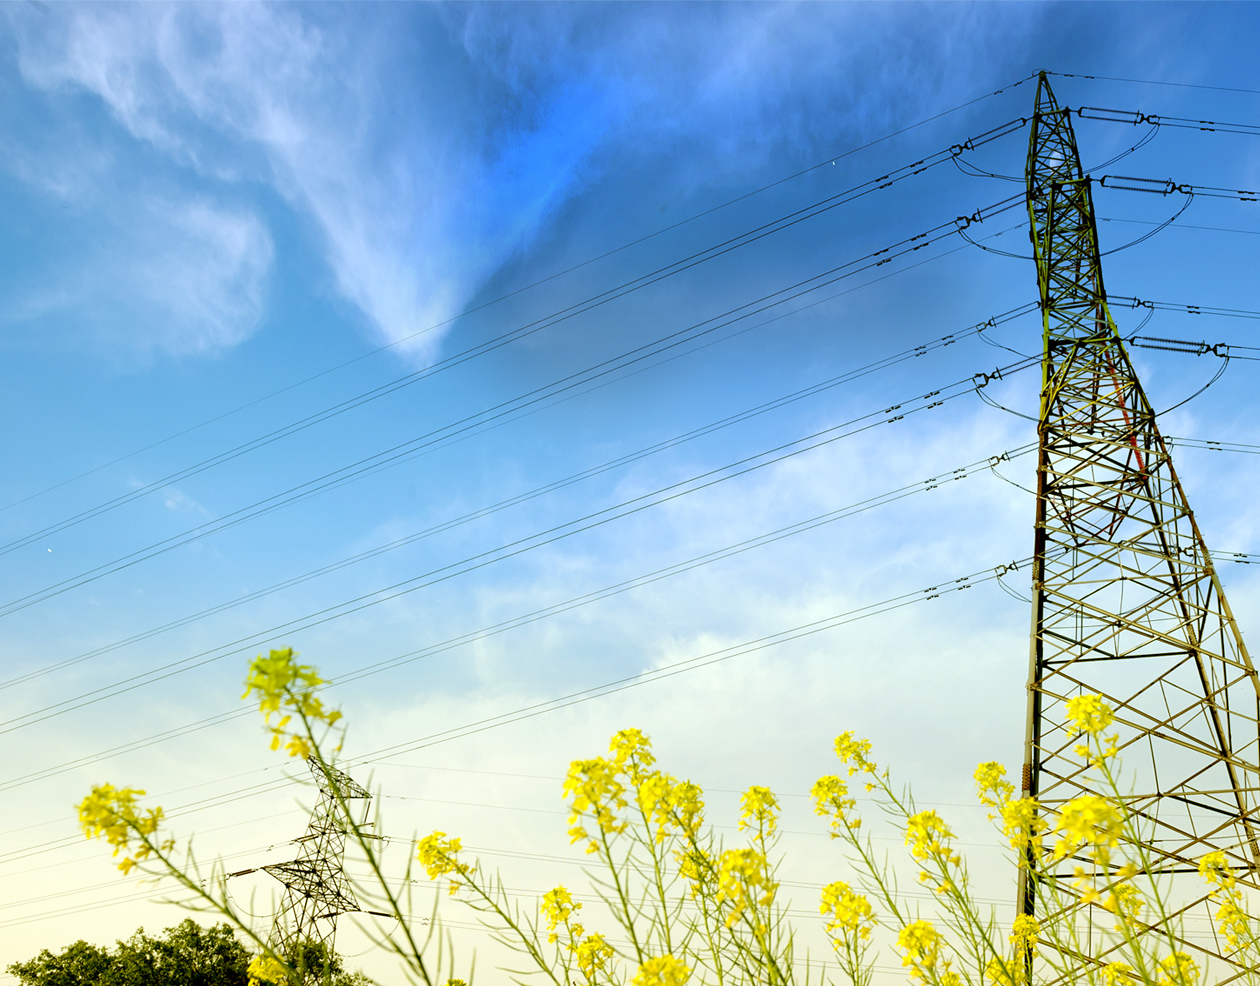
\includegraphics[scale=1]{portal-energy-background}}} % Image background

\centering
\vspace*{9cm}
\par\normalfont\fontsize{35}{35}\sffamily\selectfont
Etude et estimation de la consommation totale d'électricité par calage avec ou sans réduction du nombre de variables auxiliaires.\par % Book title
\vspace*{1cm}
{\Huge Amin El Gareh et Cheikh Med Lmami Bezeid}\par % Author name
\endgroup

%---------------------------------------------------


\chapterimage{background.pdf} % Chapter heading image


\renewcommand\contentsname{Table des Matières}
\tableofcontents

%----------------------------------------------------------------------------------------
%	CHAPTER 1
%----------------------------------------------------------------------------------------


\chapterimage{chapter_head_1.pdf} % Chapter heading image


\chapter{Présentation des données d'électricité}

\section{Introduction des données}

On s’intéresse à des données d'électricité irlandaise de très grandes dimensions. Il s'agit de la consommation d'électricité enregistrée toutes les 30 minutes pendant 2 semaines (du lundi 5 octobre 2009 à 00:00 au dimanche 18 octobre 2009 à 23h30) pour 6291 individus: résidentiels, petites \& moyennes entreprises, et autres.
Ces données sont des données fonctionnelles car elles sont constituées d’un certain nombre de valeurs discrètes qui ont été mesurées, enregistrées par le CER (Commission for Energy Regulation ), mais dont l’ensemble reflète une variation régulière. Comme en théorie, on pourrait obtenir une grande quantité de points, aussi rapprochés que l’on veut, on voit que l’on obtient une courbe et que l’on peut traiter la donnée comme une fonction.

%------------------------------------------------

\section{Etude descriptive des données}

Notre objectif ici est d'isoler le ou les comportements de consommation d'un ensemble d'individus appartenant à une même classe: résidentiels, petites \& moyennes entreprises, ou autres. 

\subsection{Consommation moyenne}
On considère la consommation moyenne comme étant la consommation totale prise en moyenne sur toute la population et par jour de la semaine. Sur la figure 1.1, on a représenté cette consommation moyenne en fonction du temps en minutes, et les jours de la semaine y sont délimités par des traits verticals rouges. 
L'analyse de la courbe des individus "résidentiels" et "autres", nous révèle le caractère cyclique de la consommation moyenne sur une période de 24h. La courbe des individus "petites \& moyennes entreprises" indique une consommation moyenne qui s'apparente être cyclique entre le lundi et le vendredi, mais qui ne l'est pas le week-end.


%-----------------------------------------------

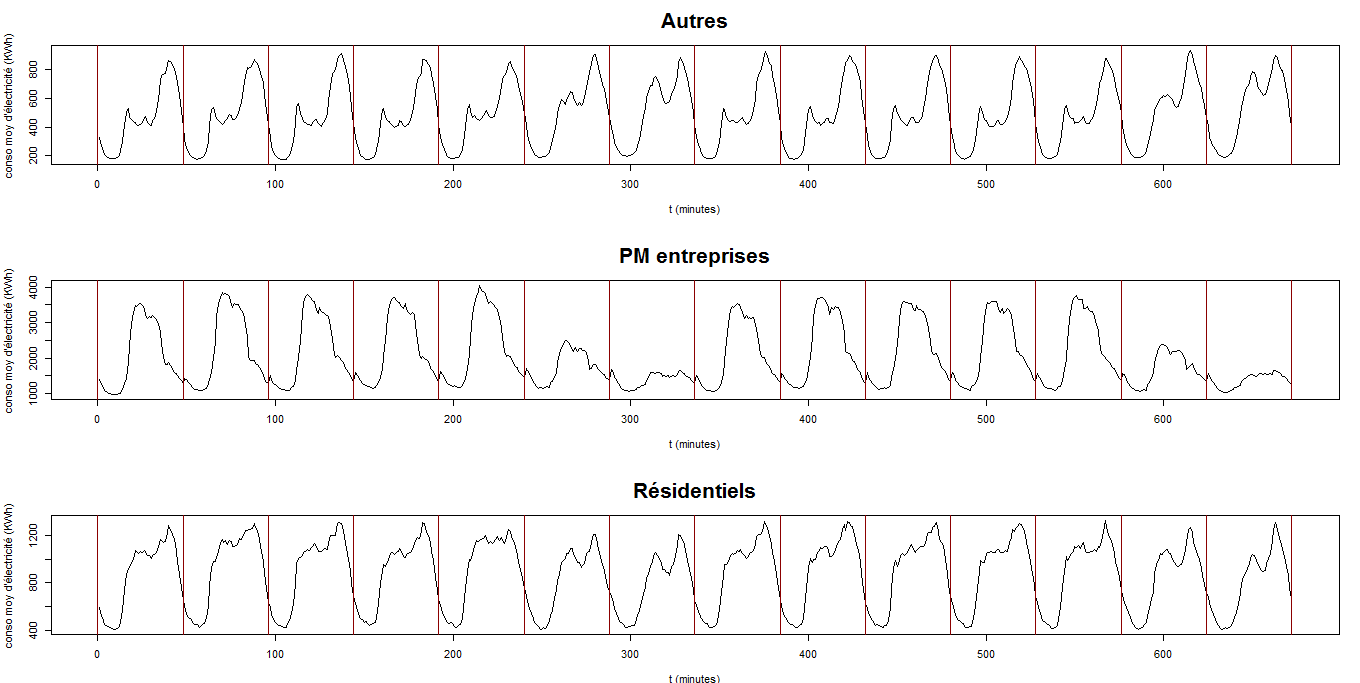
\includegraphics[scale=0.45]{Rplot_A}
 \begin{center} Figure 1.1 - Courbes de la consommation moyenne en fonction du temps (en minutes) \end{center}


\subsection{Mesure de la dispersion}
L'illustration 1.2 met en relation la variance de la consommation des individus avec la classe d'appartenance. On peut distinguer un écart important entre les variances des petites \& moyennes entreprises et les autres classes.  


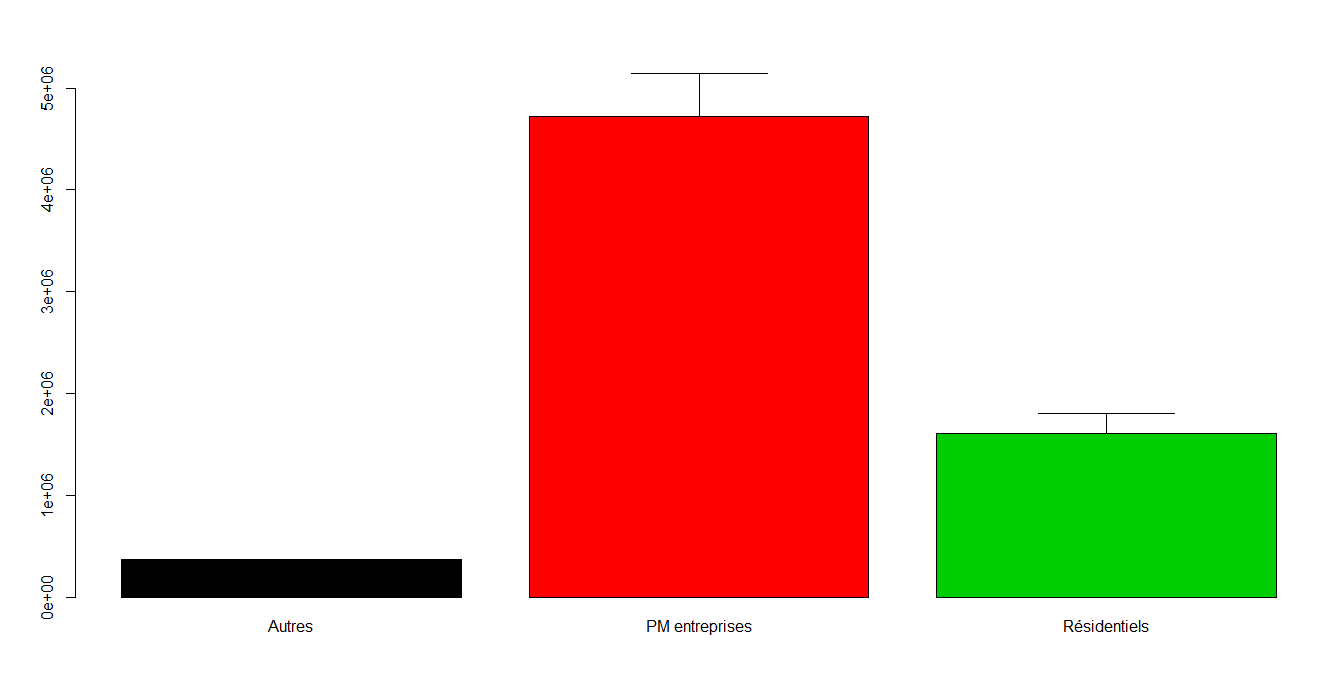
\includegraphics[scale=0.4]{Rplot_C}
 \begin{center} Figure 1.2 -  Diagrammes en colonnes : variance de la consommation des individus par classes  \end{center}
 
%-----------------------------------------------

\newpage 
 
Etudier la répartition journalière des boîtes à moustaches (n\textsuperscript{o}1: lundi 5 octobre, ... , n\textsuperscript{o}14: dimanche 18 octobre) permet d'abord de confirmer l'intuition que nous avions concernant la consommation moyenne journalière d'électricité qui s'avère être effectivement régulière. De plus, la figure 1.3 indique la présence d'un nombre important d'individus atypiques, en particulier "résidentiel", et qui par conséquent peuvent être problématique
car ils peuvent biaiser les résultats, notamment pour la variance intra-classe.

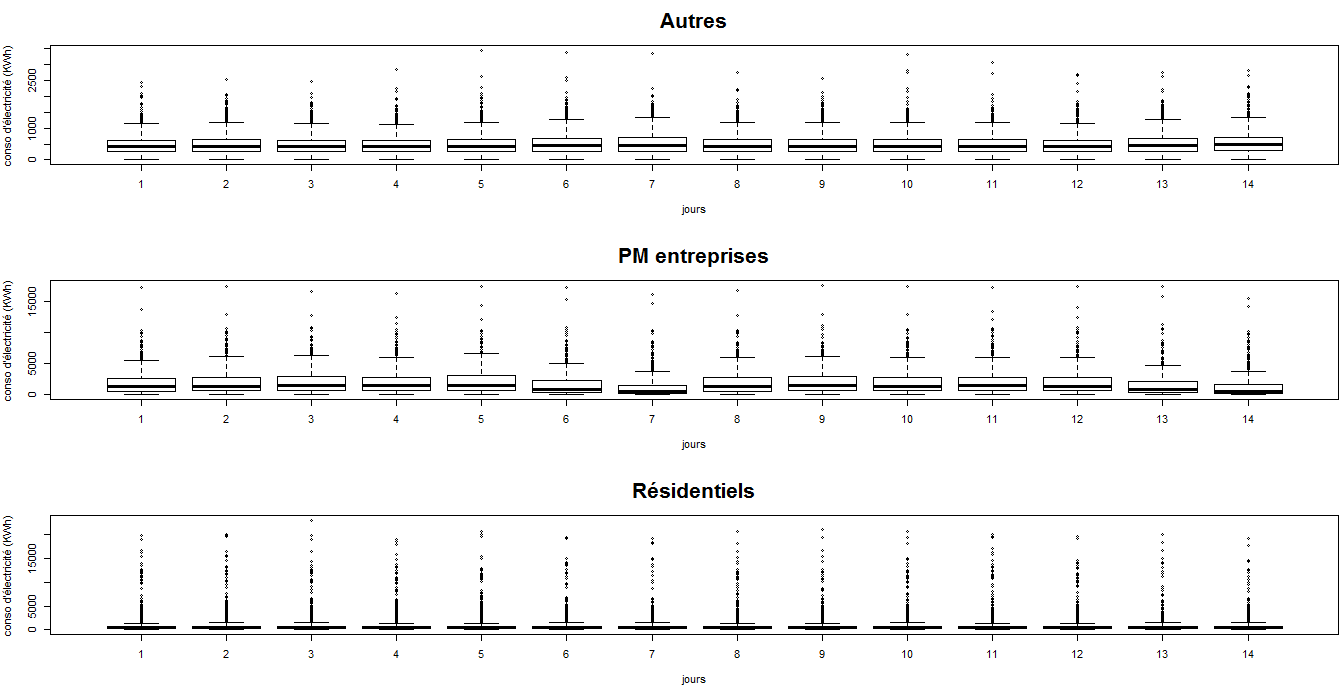
\includegraphics[scale=0.45]{Rplot_B}
 \begin{center} Figure 1.3 - Boîtes à moustaches de la consommation des individus par jour \end{center}

\subsection{Analyse en composantes principales}

La première étape consiste à sélectionner le nombre d’axes factoriels. En utilisant le critère de Kaiser, nous sélectionnons les 3 premières valeurs propres qui expliquent 72.72\% de l’inertie totale du nuage de points. Néanmoins, comme le troisième axe n’est corrélé significativement qu’avec une seule variable, nous ne le considérons pas dans l’interprétation.


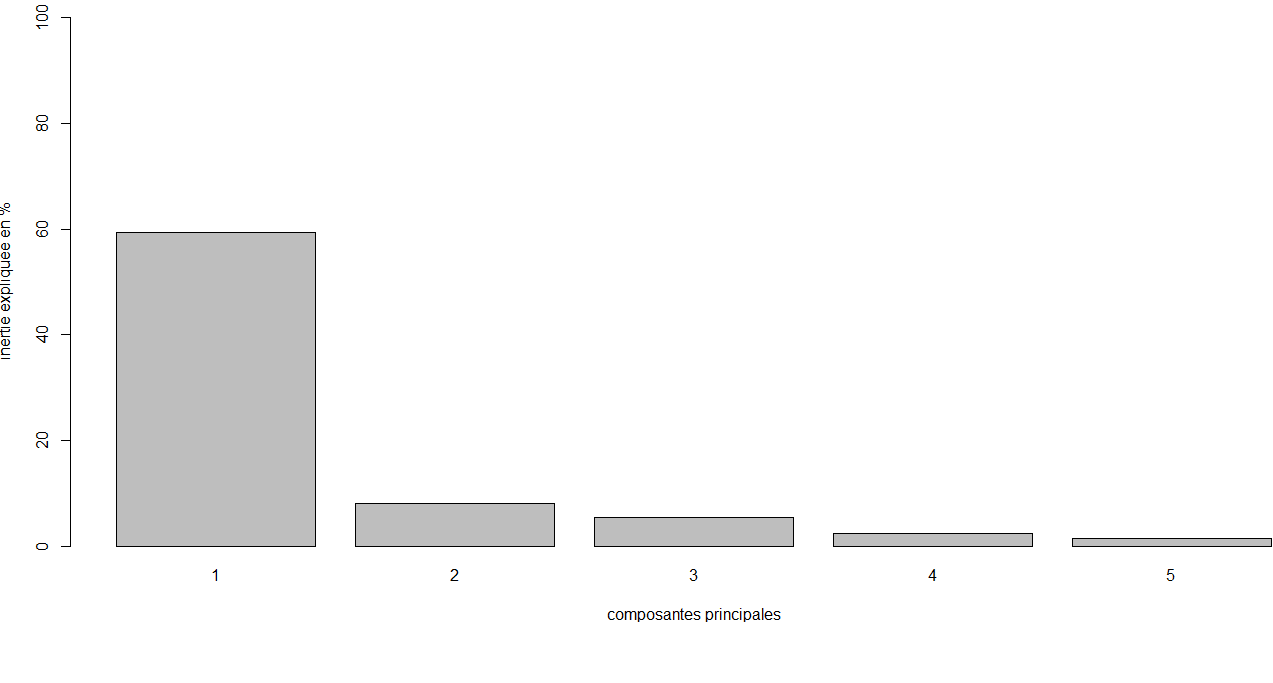
\includegraphics[scale=0.40]{Rplot_D}
 \begin{center} Figure 1.4 - Part de l'inertie  \end{center}
 
Le cercle des corrélations pour le plan formé des deux premiers axes factoriels est représenté figure 1.5 et 1.6. Toutes les  variables sont bien représentées dans ce plan factoriel puisqu'elles sont proches du bord du cerle de corrélation. Sur la figure 1.5 on a choisi de prendre les variables représentatives d'un jour entre le lundi et le samedi, soit le vendredi 9 octobre 2009, et pour une meilleure visibilité nous avons divisé la représentation des variables en deux parties: matin-midi et midi-soir. Tandis que sur la figure 1.6 nous avons pris les variables représentatives du dimanche 11 octobre 2009.  

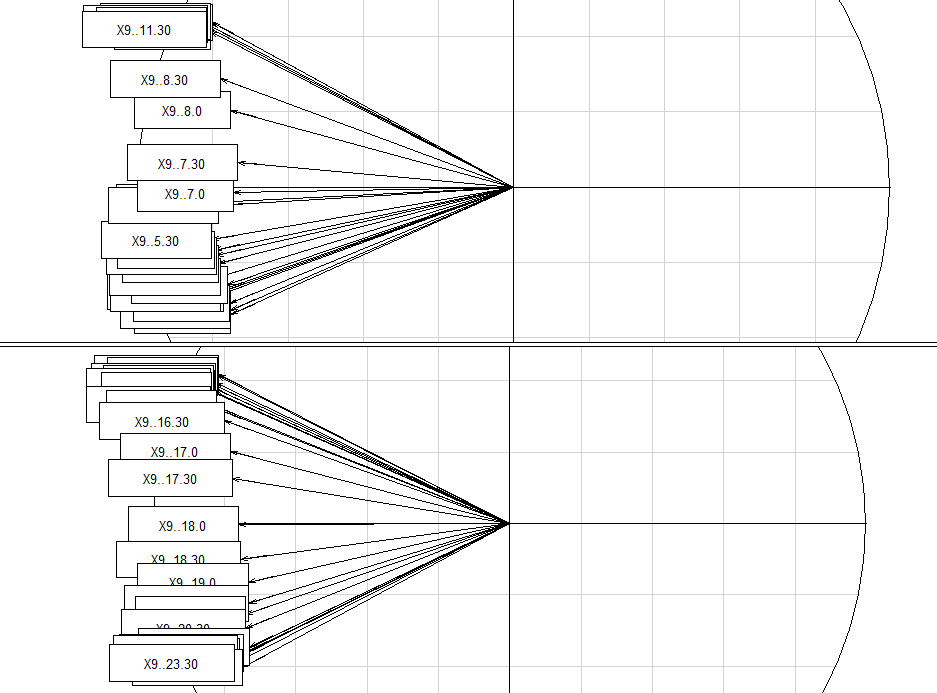
\includegraphics[scale=0.50]{Rplot_E}
 \begin{center} Figure 1.5 - Cercle des corrélations, représentation des variables du vendredi 9 octobre 2009 \end{center}
 
 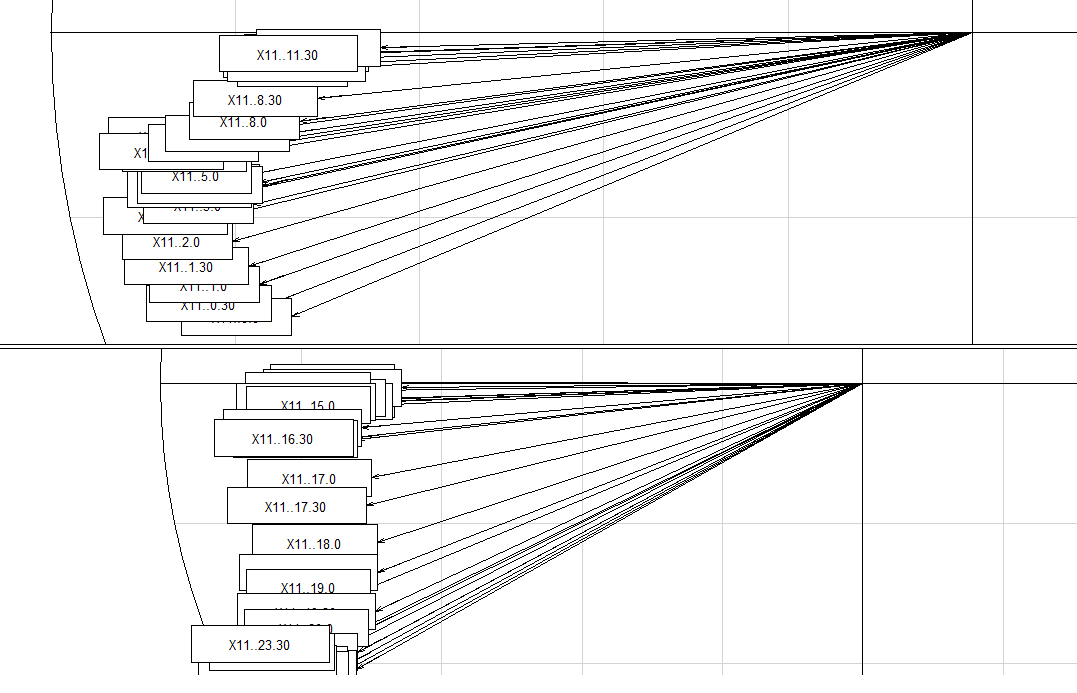
\includegraphics[scale=0.50]{Rplot_F}
 \begin{center} Figure 1.6 - Cercle des corrélations, représentation des variables pour le dimanche 11 octobre 2009 \end{center}

  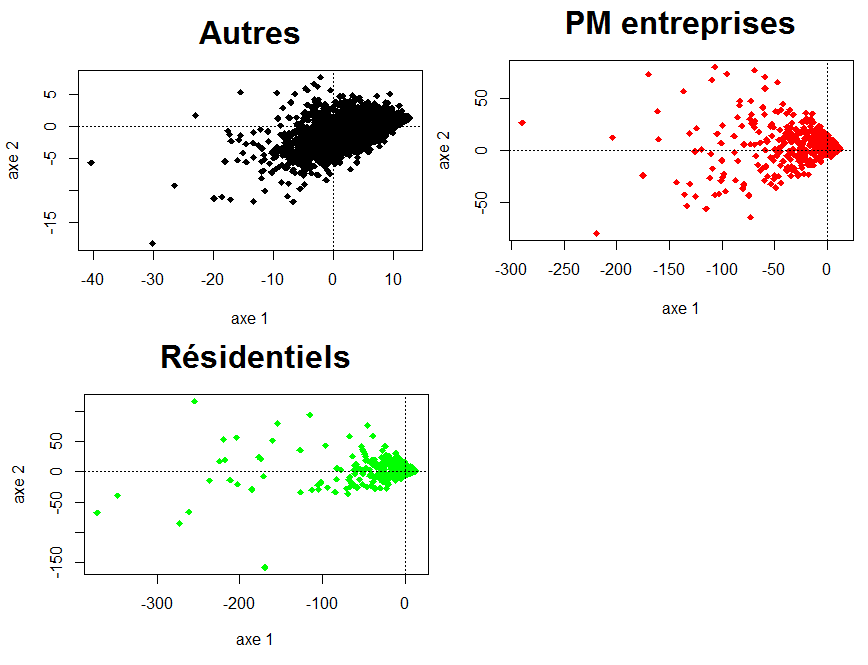
\includegraphics[scale=0.55]{Rplot_G}
 \begin{center} Figure 1.7 - Représentation des individus dans le plan factoriel selon la classe d'appartenance \end{center}
 
 \vspace{4em}
 
 On constate que les variables entre 8h et 18h sont bien représentées par rapport au premier axe tandis que le reste des variables est moins bien représenté. On peut donc dire que ce dernier explique la consommation d'électricité.
 
 \vspace{1em}
 
En utilisant une approche simultanée entre les graphes des individus et des variables, on s'aperçoit que tous les individus sont bien représentés par rapport au premier axe. Par conséquent, ces mêmes individus ont des valeurs élevées pour les variables entre 8h et 18h.
 
 \vspace{1em}
 
 Pour le cas particulier du dimanche, on constate que les variables sont toutes négativement corrélés au deuxième axe. Cet axe explique la consommation, qui s'avère être faible.
 
 
 
%------------------------------------------------

%----------------------------------------------------------------------------------------
%	CHAPTER 2
%----------------------------------------------------------------------------------------

\chapterimage{chapter_head_1.pdf} % Chapter heading image

\chapter{Présentation du calage}


En théorie des sondages, nous sommes souvent confrontés à l'estimation du total d'une variable d'intérêt Y

\begin{align*}
&  t_{y}=\sum_{k\in U} y_k  
\end{align*}

\section{Estimation par Horvitz-Thompson}

Horvitz et Thompson (1952) ont présenté un estimateur linéaire sans biais d'un total $t_y$ valable pour tout plan de sondage

\begin{align*}
&  \hat{t_{y}}=\sum_{k\in s} \frac{y_k}{\pi_k}  
\end{align*}


Cet estimateur est appelé le $\pi$-estimateur ou estimateur de Horvitz-Thompson. En effet, les valeurs prises par le caractère y sur les unités de l'échantillon sont dilatées par l'inverse des probabilités d'inclusion.\\


\begin{theorem}
Si $\pi_k$ > 0, $k\in$ U, alors $\hat{t_y}$ estime $t_y$ sans biais. 
\end{theorem}



\textit{Demonstration.}

\begin{align*}
& \mathbb{E}[\hat{ty}] \:\:\:\:=\:\: \mathbb{E}\left[ \sum_{k\in s} \frac{y_k}{\pi_k} \right]\\
& \quad\quad\quad =\:\: \mathbb{E}\left[ \sum_{k\in U} \frac{I_k y_k}{\pi_k} \right] \quad \textnormal{ où } I_k \: \textnormal{ est une variable indicatrice qui vaut 1 si } k\in s \textnormal{ et } 0 \textnormal{ sinon}\\
\end{align*}


%------------------------------------------------

\newpage

\begin{align*}
& \quad\quad\quad =\:\: \sum_{k\in U} \frac{\mathbb{E}[I_k] y_k}{\pi_k}\\
& \quad\quad\quad =\:\: \sum_{k\in U} yk\\
& \quad\quad\quad =\:\: t_y\\
& \textnormal{Par conséquent, }\: Biais(\hat{ty})=\mathbb{E}[\hat{ty}]-ty=0\quad\quad\quad \blacksquare
\end{align*}


%------------------------------------------------

\section{Estimation par calage}

Les méthodes de calage ont été formalisées par Deville et Särndal (1992). ils donnent un cadre général pour l'estimation par calage et étudient les propriétés de ces estimateurs. L'information auxiliaire utilisée est un vecteur de totaux connus $t_{x}$. 

\begin{definition}[Estimateur de calage]
La méthode de calage consiste à chercher de nouveaux coefficients de pondération à affecter aux variables.
L'estimateur par calage du total est un estimateur linéaire homogène qui s'écrit:

\begin{align*}
&  \hat{t}_{w,y}=\sum_{k\in s} w_{ks}y_k
\end{align*}
\end{definition}

\begin{proposition}[]
Les poids $w_{ks}$ dépendent de l'échantillon aléatoire et sont déterminés de sorte que l'estimateur soit calé sur les totaux des caractères auxiliaires.   
\begin{align*}
&  \hat{t}_{wx}=t_x \quad \textnormal{ où } \quad \hat{t}_{wx}=  \sum_{k\in s} w_{ks}x_k
\end{align*}
\end{proposition}

\begin{notation}
Par commodité on pose $w_k=w_{ks}$, pour tout $k\in s$
\end{notation}

\vspace{1em}

\begin{remark}
Comme il existe une infinité de poids $w_k$ qui satisfait la proposition 2.2.1, on va chercher des poids proches des poids $ \pi_k^{-1}$ du $\pi$-estimateur. Notons:
\begin{align*}
&  d_k=\frac{1}{\pi_k} ,\quad k\in s  
\end{align*}
\end{remark}

\vspace{1em}

\begin{theorem}
Si $\pi_k$ > 0, $k\in$ U, alors $\hat{t_{wy}}$ estime asymptotiquement sans biais $t_y$ 
\end{theorem}


\textit{Demonstration.}

\begin{align*}
& \textnormal{Le choix des poids wk proches de $d_k$ assure la convergence asymptotique de l'estimateur de calage $\hat{t_{wy}}$}\\ 
& \textnormal{vers l'estimateur de Horvitz-Thompson $\hat{t_y}$ }\\
& \sum_{k\in s} w_k x_k \rightarrow \sum_{k\in s} d_k x_k \Leftrightarrow \hat{t_{wy}} \:\: \rightarrow \:\: \hat{t_y}\\ 
& \textnormal{Comme $ \hat{t_{wy}}$ est uniformement bornée car c'est une somme finie alors, on a:}\\
& \hat{t_{wy}} \:\: \rightarrow \:\: \hat{t_y} \Rightarrow
\mathbb{E}[\hat{t_{wy}}] \:\: \rightarrow \:\: \mathbb{E}[\hat{t_y}]\\
& \textnormal{Par conséquent, } \: Biais(\hat{t_{wy}}) \:\: \rightarrow \:\: \mathbb{E}[\hat{t_y}]-t_y=0 \quad\quad\quad \blacksquare
\end{align*}

%------------------------------------------------

\newpage 

Pour garantir le critère de proximité entre $w_k$ et $d_k$, on va utiliser une pseudo-distance de Khi-deux, $ F_k(w_k,d_k)=\frac{(wk-dk)^2}{dk}$.\\ 
La fonction $F_k(w_k,d_k)$ est supposée positive, dérivable par rapport à $w_k$ et strictement convexe, telle que $F_k(w_k,d_k)=0$. Les poids $w_k,\: k\in s$, sont obtenus en résolvant le problème $(P)$ de minimisation

\begin{equation*}
(P) :=\left\{\begin{aligned} & \sum_{k\in s} F_k(w_k,d_k)=\sum_{k\in s} \frac{(w_k-d_k)^2}{d_k} \leftarrow \textbf{min}\\
 \\ & \hat{t}_{wx_j}=t_{x_j}  \quad\quad\quad\quad j=1,...,p \end{aligned}\right.
\end{equation*}


On peut écrire la fonction Lagrangienne :
\begin{align*}
&  L(w_k,\lambda_j) \:\:= \sum_{k\in s} \frac{(w_k-d_k)^2}{d_k}-\sum_{j=1}^p \lambda_j(\hat{t}_{wx_j}-t_{x_j})\\ 
& \quad\quad\quad\quad = \sum_{k\in s} \frac{(w_k-d_k)^2}{d_k}-\sum_{j=1}^p \lambda_j\left(\sum_{k\in s} w_k x_{k_j} -  \sum_{k\in U}x_{k_j}\right)
\end{align*}

où les $\lambda_j$ sont les multiplicateurs de Lagrange. En annulant les dérivées partielles du Lagrangien par rapport aux $w_k$, on obtient: 

\begin{align*}
&  \frac{\delta L(w_k,\lambda_j)}{\delta w_k}=0 \:\:\:\:\:\:	\Leftrightarrow\:\: 2\left(\frac{w_k-d_k}{d_k}\right)-\sum_{j=1}^p \lambda_j x_{k_j}=0 
\end{align*}


\begin{align}
& \quad\quad\quad\quad\quad\quad\quad\: \Leftrightarrow \:\: w_k=d_k\left( \frac{1}{2} \sum_{j=1}^p \lambda_j x_{k_j} +1 \right) 
\end{align}


En considérant l'expression des poids $w_k$ et d'après les contraintes de $(P)$, on obtient:

\begin{align*}
& t_{x_j} = \sum_{k\in s} w_k x_{k_j} \:\:  \Leftrightarrow \:\:  t_{x_j} = \sum_{k\in s} d_k  x_{k_j} \left( \frac{1}{2} \sum_{j=1}^p \lambda_j x_{k_j} +1 \right)\\
& \quad\quad\quad\quad\quad\:\:\:\:\:\: \Leftrightarrow \:\:  t_{x_j} = \sum_{k\in s} d_k  x_{k_j} +  \frac{1}{2} \sum_{k\in s} d_k  x_{k_j} \sum_{j=1}^p \lambda_j x_{k_j}
\end{align*}

L'expression peut également s'écrire sous forme matricielle


%------------------------------------------------

\begin{align*}
& t_x \:\:=\:\: \hat{t_x} +\frac{1}{2}\sum_{k\in s} d_k x_k ^t x_k \lambda
\end{align*}

Sous réserve que la matrice $\sum_{k\in s} d_k x_k ^t x_k$ soit inversible, on peut déterminer $\lambda$

\begin{align*}
\lambda\:\:=\:\:2\left( \sum_{k\in s} d_k x_k ^t x_k \right)^{-1}(t_x-\hat{t_x})
\end{align*}

En remplaçant $\lambda$ dans l'expression (2.1) on obtient les poids $w_k$

\begin{align}
& w_k\:\:=\:\:d_k\left(\frac{1}{2}\: ^t\lambda x_k +1\right)\:\: = \:\: d_k \left( ^t(t_x-\hat{t_x}) \left( \sum_{k\in s} d_k x_k ^t x_k \right)^{-1} x_k + 1 \right)
\end{align}

Enfin, l'estimateur de calage $ \hat{t_{wy}} \:\:=\:\:\sum_{k\in s} w_k y_k$ peut s'écrire

\begin{align}
&  \hat{t_{wy}} \:=\: \hat{t_y} + ^t(t_x-\hat{t_x}) \left( \sum_{k\in s} d_k x_k ^t x_k \right)^{-1}  \sum_{k\in s} x_k d_k y_k
\end{align}


\section{Application du calage}

On souhaite estimer la consommation totale d'électricité de la deuxième semaine, $t_y=1485176258$. Il y'a 336 variables auxiliaires, qui représentent les consommations  prises toutes les 30 minutes pendant la première semaine. Et sont présentées dans les vecteurs   $(t_{x_j})_{j=1,...,336} \:=\: \sum_{k\in U} x_{k_j}$. 

\subsection{Calage selon un plan SAS}

Soit U la population d'étude composée de N=6291 individus qui consomment de l'électricité sur deux semaines consécutives. La première approche consiste à sélectionner un échantillon s $\subset$ U selon un plan de sondage p(.) aléatoire simple sans remise (SAS) de taille n=600.

\begin{definition}
Un plan de taille fixe n est dit simple sans remise (SAS) si et seulement si
\begin{equation*}
p(s) :=\left\{\begin{aligned} & \binom{N}{n}^{-1} \quad \textnormal{si card(s)\:=\:n}\\
 \\ & \:\: 0  \quad\quad\quad\: \textnormal{ sinon} \end{aligned}\right.
\end{equation*}
\end{definition}

\begin{definition}
Les probabilités d'inclusion d'ordre un peuvent être déduites du plan de sondage p(.) SAS

\begin{equation*}
\pi_k=\sum_{k\in s} p(s)=\sum_{k\in s} \binom{N}{n}^{-1} = \binom{N-1}{n-1}\binom{N}{n}^{-1}=\frac{n}{N}, \textnormal{ pour tout k} \in \textnormal{ U}
\end{equation*}
\end{definition}

\begin{remark}
Les probabilités d'inclusion associées à nos données sur l'électricité sont $\pi_k=\frac{600}{6291}$.
\end{remark}


%------------------------------------------------

\newpage

On a simulé I=500 échantillons aléatoires simples sans remise de taille n=600, en utilisant la méthode de calage présentée au paragraphe 2.2 on obtient une estimation moyenne de $\bar{\hat{t}}_{wy}=\frac{1}{I}\sum_{i=1}^I \hat{t}_{wy}^{(i)}=1492219885$.\\

Pour comparer l'estimateur de Horvitz-Thompson avec celui par le calage on utilise le rapport des variances $R$ qui suit:

\begin{equation*}
R=\frac{Var(\hat{t_{wy}})}{Var(\hat{t_y})}\approx\frac{\sum_{i=1}^{I} (\hat{t_{wy}}^{(i)}-t_y)^2}{\sum_{i=1}^{I} (\hat{t_y}^{(i)}-t_y)^2}=\frac{1.747882e+17}{3.690269e+18}= 0.047365
\end{equation*}
 
La même précision est obtenue en utilisant le calage avec un plan SAS de taille n\:=\:600*0.047365\:=\:29 qu'en prennant la méthode de Horvitz-Thompson avec un plan SAS de taille n\:=\:600.\\


Le coefficient de variation $c_v$ est une mesure de dispersion relative, qui va être utilisé comme contrôle de qualité pour l'estimateur de calage.

\begin{equation*}
 c_v=\frac{\sqrt{Var(\hat{t_{wy}})}}{\bar{\hat{t_{wy}}}} = 0.011618 \quad \textnormal{ qui peut aussi s'exprimer en pourcentage, soit cv\:=\: 1.1618\%}
 \end{equation*}
 
 
 
 \subsection{Calage selon un plan Stratifié avec SAS}
 
 
 
\vspace{1em}

 Notre population d'étude $U$ est divisée dans $H=3$ strates avec $N_h$ unités dans la strate $h$.\\ 
 Les tailles des strates sont connues et valent $N_1=4225$ pour la strat "Autres", $N_2= 485$ pour la strat "P\&M entreprises", et $N_3=1581$ pour la strat "Résidents". Et vérifient la condition suivantes: $N_1+N_2+N_3=N=6291$
 
 
\vspace{1em}

 La deuxième approche pour sélectionner notre échantillon $s$ sera d'appliquer le plan SAS dans chacune des trois strates.
 
 
\vspace{1em}

 Pour trouver le nombre d'unités échantillonnées $n_h$ dans chaque strate on utilise une allocation proportionnelle: $\frac{n_h}{N_h}=\frac{n}{N}$.
 
 \vspace{1em}
 
L'estimateur de Horvitz-Thompson selon le plan Stratifié pour le total $t_y$ est donné par: 
  
  \begin{equation*}
 \hat{t_{str}}=\sum_{h=1}^H \frac{N_h}{n_h} \sum_{k\in s_h} y_k.
   \end{equation*}
   
 \vspace{1em}  

Et l'estimateur de calage selon le plan Stratifié est de:
  
  \begin{equation*}
  \hat{t_{wstr}}=\sum_{h=1}^H w_{k,s_h} \sum_{k\in s_h} y_k.
   \end{equation*}
   
  
\newpage
  
On a simulé $I=500$ échantillons tirés selon le plan Stratifié avec SAS chacun de taille $n=600$.
On obtient une estimation moyenne de $\bar{\hat{t_{wstr}}}=1504942728$.

\vspace{1em}

Pour comparer l'estimateur de Horvitz-Thompson avec celui du calage pour ce plan on calcule  \begin{equation*}
R=\frac{Var(\hat{t_{wstr}})}{Var(\hat{t_{str}})}\approx\frac{\sum_{i=1}^{I} (\hat{t_{wstr}}^{(i)}-t_y)^2}{\sum_{i=1}^{I} (\hat{t_{str}}^{(i)}-t_y)^2}= 0.231561
\end{equation*}  

La même précision est obtenue en utilisant le calage par Stratification avec SAS de taille n\:=\:600* 0.231561\:=\:139 qu'en prennant la méthode de Horvitz-Thompson avec un plan SAS de taille n\:=\:600.\\

On calcule le coefficient de variation $c_v$, qui vaut:

\begin{equation*}
 c_v=\frac{\sqrt{Var(\hat{t_{wstr}})}}{\bar{\hat{t_{wstr}}}} = 0.02203803 \quad \textnormal{ qui peut aussi s'exprimer en pourcentage, soit cv\:=\: 2.203803\%}
 \end{equation*}
 

\begin{remark}
Le calage qui a été effectué suivant l'un ou l'autre des plans utilise une pseudo-distance de khi-deux. Cette pseudo-distance est à l'origine de l'obtention de poids négatifs.\\ 
Pour y remédier on peut utiliser d'autres méthodes comme logistique, raking ratio, linéaire tronquée, ...  
\end{remark}

 
 
 

%------------------------------------------------

%----------------------------------------------------------------------------------------
%	CHAPTER 3
%----------------------------------------------------
\chapterimage{chapter_head_1.pdf} % Chapter heading image

\chapter{Présentation du calage sur CP}


Le calage en présence de beaucoup de variables auxilaires peut s'avérer instable surtout s'il y'a des collinéarités entre les variables auxiliaires. Une méthode pour palier cet incovénient est de réduire l'information auxiliaire en réalisant une ACP.

\section{Méthode de calage sur CP}

\subsection{Information auxiliaire sur CP}

Soient $\lambda_1\ge \lambda_2\ge ... \ge \lambda_p > 0$ les valeurs propres de matrice de variance-covariance $\frac{1}{N}X^{T}X$, où $X$ est la matrice formée des vecteurs $(X_j)_{1,...,p}$ contenant l'information auxiliaire de départ. Et soient $v_1,...,v_p$ les vecteurs propres associés aux $(\lambda_j)_{j=1,...,p}$.

\vspace{1em}

Les composantes principales \: $Z_1,...,Z_p$ \: qui sont les combinaisons linéaires des $(X_j)_{1,...,p}$ \\
sont définies par la relation  \: $Z_j=X v_j, \quad\quad j=1,...,p$.

\vspace{1em}

On va sélectionner selon le critère de Kaiser les r premières composantes principales, qui vont formées les nouvelles variables auxiliaires. La matrice d'information auxiliaire est maintenant donnée par: 

\begin{align*}
& Z=(Z_1,...,Z_r)=(z_k)_{k\in U} \quad\quad \textnormal{où } \quad z_k=(z_{k1},...,z_{kr})^{T} 
\end{align*}

\subsection{Calage sur CP}


Notre objectif est de trouver les poids de calage $(w_k)_{k\in s}$ qui vérifient:

\begin{equation*}
(P') :=\left\{\begin{aligned} & \sum_{k\in s} F_k(w_k,d_k)=\sum_{k\in s} \frac{(w_k-d_k)^2}{d_k} \leftarrow \textbf{min}\\
 \\ & \hat{t}_{wz_j}=t_{z_j}  \quad\quad\quad\quad j=1,...,r \end{aligned}\right.
\end{equation*}

\begin{remark}
Les équations de calage qui peuvent aussi s'écrire sous la forme \:\:
$\sum_{k\in s} w_k z_{k_j}=\sum_{k\in s} z_{k_j}$\\
\: où $ \hat{t}_{wz_j}=\sum_{k\in s} w_k z_{k_j}$ est un estimateur dépendant du paramètre $r$ 

\begin{enumerate}
\item[-]  Si $r=0 $ on obtient l'estimateur de Horvitz-Thompson $\hat{t_y}$ qui n'utilise pas l'information auxiliaire.
\item[-] Si $r=p $ on obtient l'estimateur calé sur les $p$ variables de départ.
\end{enumerate}

\end{remark}


La résolution du problème de minimisation $(P')$ est la même que celle présentée au paragraphe 2.2, les poids $w_k$ sont donc:


\begin{align*}
& w_k\:\:=\:\:d_k\left(\frac{1}{2}\: ^t\lambda z_k +1\right)\:\: = \:\: d_k \left( ^t(t_z-\hat{t_z}) \left( \sum_{k\in s} d_k z_k ^t z_k \right)^{-1} z_k + 1 \right)
\end{align*}


Et l'estimateur de calage $ \hat{t_{wy}} \:\:=\:\:\sum_{k\in s} w_k y_k$ peut s'écrire

\begin{align*}
&  \hat{t_{wy}} \:=\: \hat{t_y} + ^t(t_z-\hat{t_z}) \left( \sum_{k\in s} d_k z_k ^t z_k \right)^{-1}  \sum_{k\in s} z_k d_k y_k
\end{align*}


\section{Application du calage sur CP}

On souhaite toujours estimer la consommation totale d'électricité de la deuxième semaine,\\
$t_y=1485176258$. La matrice des variables auxiliaires de départ $X$ est de dimension \\
$6291$ x $336$. On rappelle que la nouvelle matrice  des variables auxiliaires $Z=\left( Z_1,...,Z_r \right)$, dépend d'un paramètre $r$, que l'on peut faire varier entre $1$ et $p=336$.  Le choix du nombre $r$ de variables auxiliaires ou autrement dit composantes principales vont permettre d'étudier la qualité de l'estimation par calage.  

\vspace{1em}

On a simulé I=500 échantillons aléatoires simples sans remise de taille n=600, en utilisant la méthode de calage sur les r=2 composantes principales on obtient une estimation moyenne de $t_y$ qui est $\bar{\hat{t}}_{wy}=\frac{1}{I}\sum_{i=1}^I \hat{t}_{wy}^{(i)} =1480138029$.\\

Le rapport des variances $R$ vaut:

\begin{equation*}
R=\frac{Var(\hat{t_{wy}})}{Var(\hat{t_y})}\approx\frac{\sum_{i=1}^{I} (\hat{t_{wy}}^{(i)}-t_y)^2}{\sum_{i=1}^{I} (\hat{t_y}^{(i)}-t_y)^2}=\frac{1.088333e+17}{3.678668e+18}=0.029585 
\end{equation*}

La même précision est obtenue en utilisant le calage sur CP avec un plan SAS de taille n\:=\:600*0.029585\:=\:18 qu'en prennant la méthode de Horvitz-Thompson avec un plan SAS de taille n\:=\:600.\\


Le coefficient de variation vaut: \quad $ cv=\frac{\sqrt{Var(\hat{t_{wy}})}}{\bar{\hat{t_{wy}}}} = 0.009377838 $  \quad \textnormal{ qui peut aussi s'exprimer en pourcentage, soit cv\:=\: 0.9377838\%}\\

On va montrer que l'estimateur du calage sur les deux premières CP est dans notre cas le meilleur estimateur. Pour se faire on a calculer l'estimateur moyen $ \bar{\hat{t_{wy}}} $, le rapport $R$ et le coefficient $c_v$ pour les CP compris entre $2$ et $336$.\\

D'après la figure 1.8, la valeur de l'estimateur moyen par calage diminue en fonction du nombre de CP retenus. Le trait horizontal rouge représente la valeur exact de la consommation total d'électricité.  

  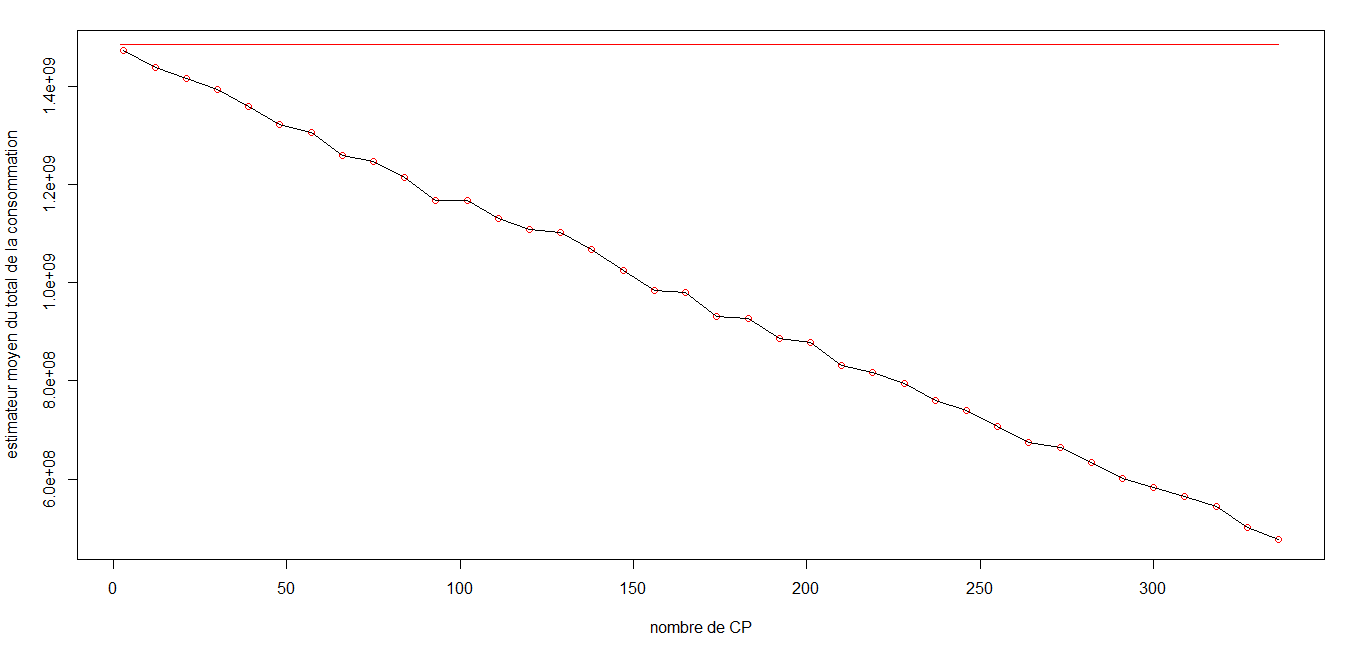
\includegraphics[scale=0.45]{Rplot_I}
 \begin{center} Figure 1.8 - Estimateur moyen $\bar{\hat{t_{wy}}}$ du total de la consommation en fonction du nombre de CP  \end{center}

\vspace{1em}

D'après la figure 1.9, le rapport des variances  $R$ évolue progressivement jusqu'à un nombre de CP égal à 200. Une fois ce nombre de CP dépassé le coefficient $R$ devient élevé et instable.

  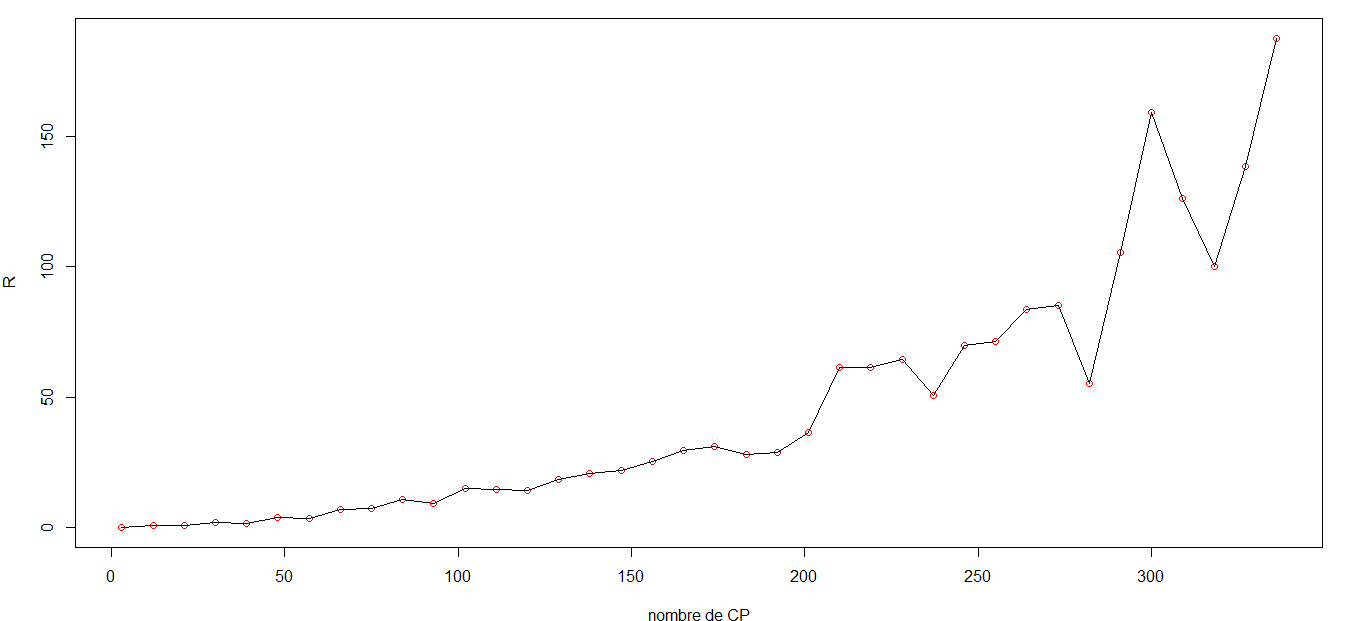
\includegraphics[scale=0.45]{Rplot_K}
 \begin{center} Figure 1.9 - Le rapport $R$ en fonction du nombre de CP \end{center}
 
 
%------------------------------------------------

 \newpage
 
 De la figure 1.10 on retiendra que le choix des 2 premières composantes principales implique une faible variation $c_v\approx 1\%$, alors que pour un nombre de CP au déla de $r=50$ le coefficient $cv$ devient relativement important (supérieur à 5\%).
 
   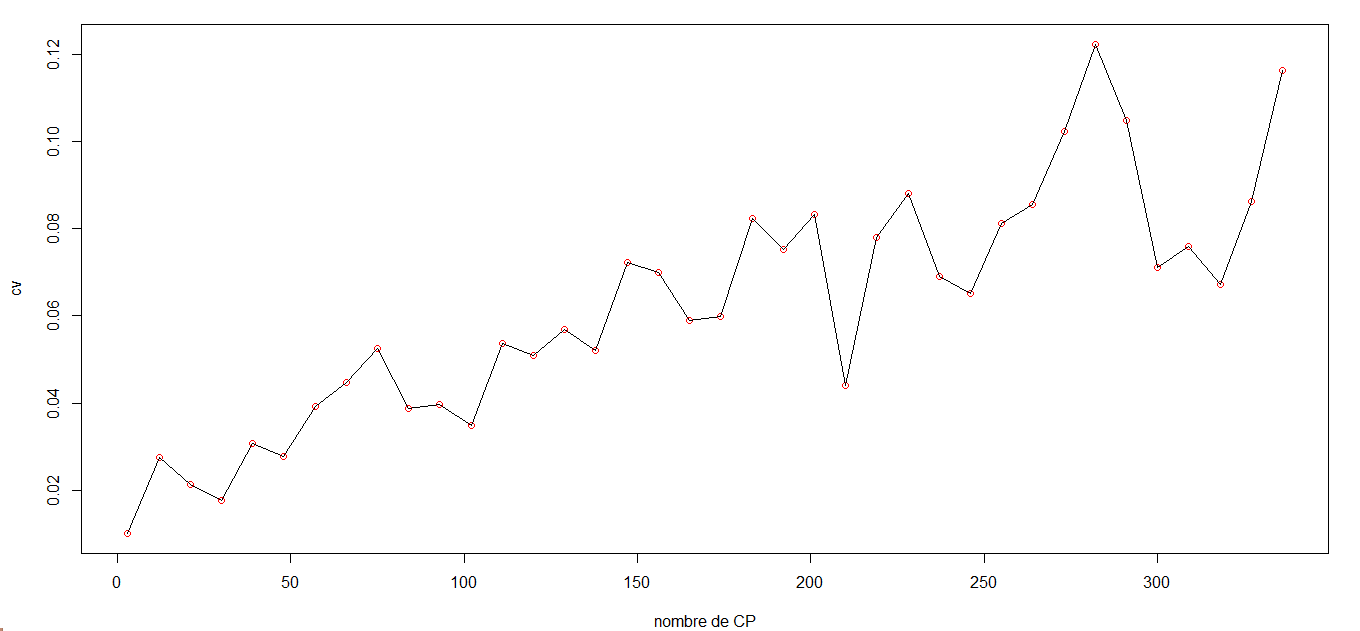
\includegraphics[scale=0.45]{Rplot_H}
 \begin{center} Figure 1.10 - Le coefficient de variation $c_v$ en fonction du nombre de CP\end{center}


\vspace{4em}

\textbf{Interprétation de la méthode du calage sur les CP}

\vspace{1em}

\textbf{$\bullet$ Avantages}

\vspace{1em}

\begin{enumerate}
\item[-] Rapide lorsque le calage est fait sur un nombre très faible de CP, car la taille de la matrice $\left( \sum_{k\in s} d_k z_k ^t z_k \right)$ à inverser est petite.
\item[-] Facile à mettre en oeuvre, elle permet d’obtenir de gains importants en termes de
variance.
\item[-] La précision R de l'estimateur de calage est meilleure par rapport aux deux autres plans, à condition que l'on retienne un nombre faible de CP.
\item[-] Le problème de positivité des poids est résolus, ceci dû au fait d'une variance répartit sur les CP.
\end{enumerate}

\vspace{1em}

\textbf{$\bullet$ Inconvénient}

\vspace{1em}

\begin{enumerate}
\item[-]Instable pour un grand nombre de CP.
\end{enumerate}

%------------------------------------------
\chapterimage{chapter_head_1.pdf} % Chapter heading image

\chapter{Présentation des programmes R}

Nous avons réalisés l'étude de la méthode de calage selon plusieurs plans:

\begin{enumerate}
\item[-] SC = Calage selon un plan SAS  (voir 2.3.1)
\item[-] SSC = Calage selon un plan Stratifié avec SAS (voir 2.3.2) 
\item[-] SAC = Calage sur Composantes principales avec SAS (voir 3.2).
\item[-] SA2C =  Calage sur les 2 premières Composantes principales avec SAS (le meilleur plan).

\end{enumerate}

\section{Organigramme}
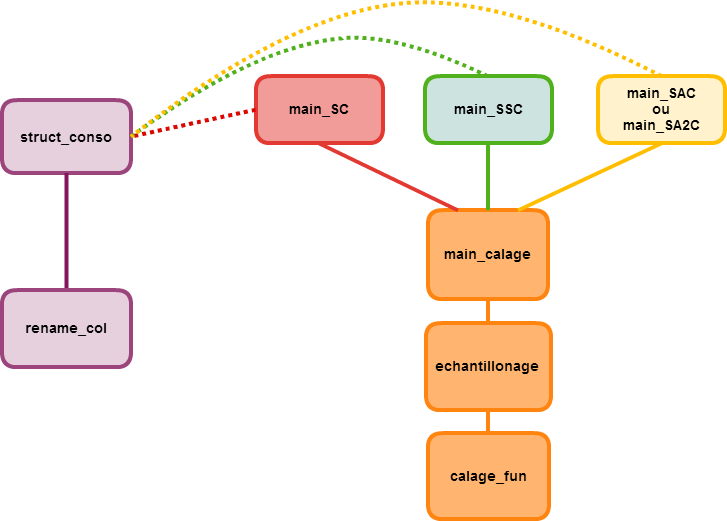
\includegraphics[scale=0.5]{Mindmap.png}

\vspace{1em}

Pour chacun des plans, on a crée un  "main" ou autrement dit un programme principal, dont les dépendances ont été généralisées. On distingue d'un côté une dépendance conditionnelle marquée par des pointillés, c'est-à-dire que struct\_conso s'exécute que si la table conso n'existe pas dans le workspace.\\ 
De l'autre côté on effectue un calage étape par étape à partir de main\_calage, qui se résume de la facon suivante:\\ 
\begin{enumerate}
\item échantillonnage selon un plan p(.) SAS avec la fonction echantillonage.
\item calcul des poids de calage avec la fonction calage\_fun. 
\item calcul des estimateurs de calage et de Horvitz-Thompson.
\end{enumerate}


\vspace{4em}

\section{Bibliothèque des programmes R}

\vspace{2em}

\verbatiminput {struct_conso.R}

\newpage

\vspace{2em}

\verbatiminput {rename_col.R}


%------------------------------------------
\newpage

\verbatiminput {main_calage.R}

%------------------------------------------
\newpage

\verbatiminput {echantillonage.R}

\verbatiminput {calage_fun.R}


%------------------------------------------
\newpage

\verbatiminput {main_SC.R}

\verbatiminput {main_SSC.R}

%------------------------------------------

\verbatiminput {main_SA2C.R}

%------------------------------------------
\newpage

\verbatiminput {main_SAC.R}

%------------------------------------------

\chapterimage{chapter_head_1.pdf} % Chapter heading image

\chapter{Conclusion}

Ce travail visait à développer plusieurs plans permettant d’estimer la consommation totale d'électricité. Introduire des méthodes issues de la théorie des sondages, nous a permis de comprendre les principes et les enjeux de cette discipline. La théorie des sondages suscite des travaux d’approfondissement récents et innovants en tout point. Du fait qu’elle porte sur des populations finies, d’existence bien concrète, elle ne peut ignorer les contraintes du monde réel. C'est dans ce sens que nous portons un intérêt pour son étude et pour son application.  



% ----------------------------------------------------------------------------------------
% 	BIBLIOGRAPHY
% ----------------------------------------------------------------------------------------

\chapter*{Bibliographie}

  1. Tillé, Y. (2001), \textit{Théorie des sondages}, chez Dunod.\\
  2. \url{http://sondages2012.ensai.fr/wp-content/uploads/2011/01/expose_rennes_gogaShehzad_20121.pdf}




%----------------------------------------------------------------------------------------

\end{document}